\begin{figure*}[t]
    % \hspace{0.04\textwidth}
    % \begin{subfigure}[b]{0.3\textwidth}
    %     \center
    %     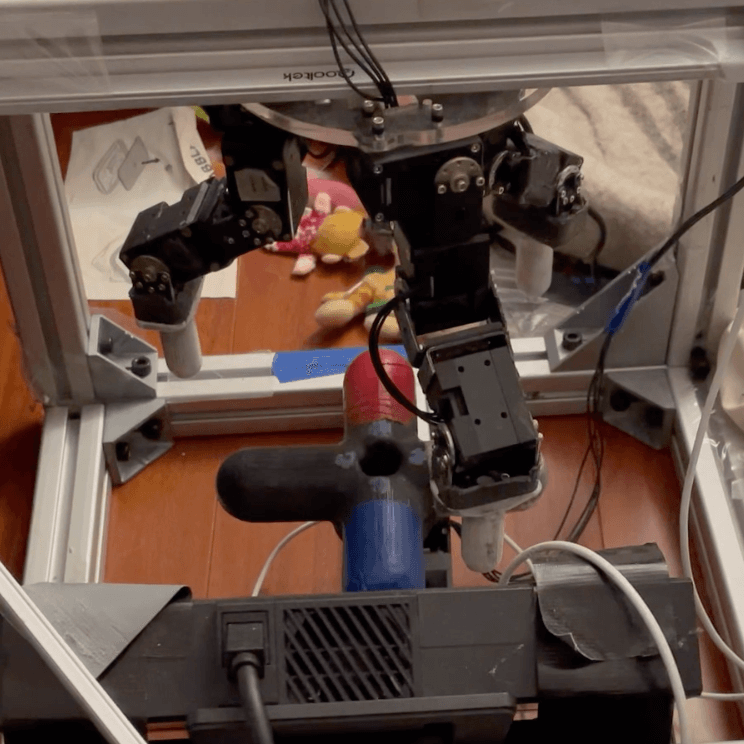
\includegraphics[height=0.6\textwidth]{awac/figures/robot/robel.png}
    %     % 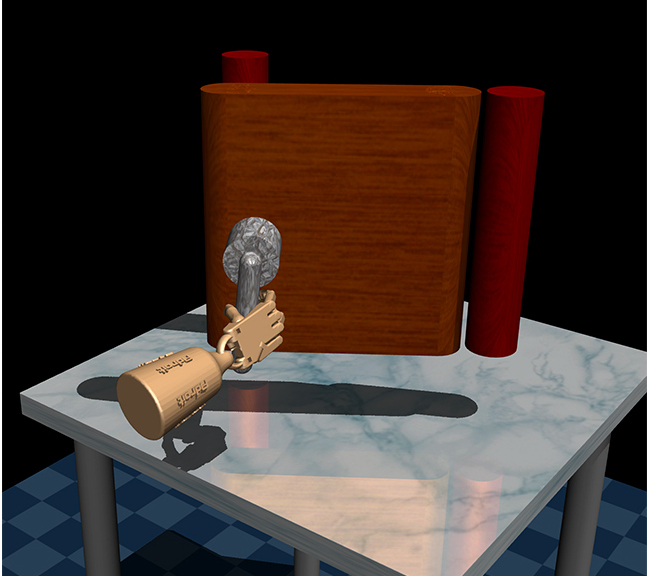
\includegraphics[height=0.26\textwidth]{awac/figures/imgs/door.jpg}
    %     % 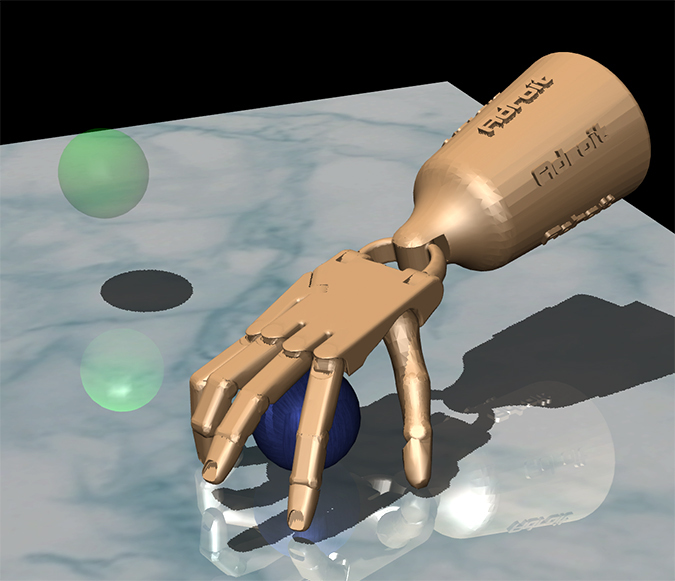
\includegraphics[height=0.26\textwidth]{awac/figures/imgs/relocate.jpg}
    % \end{subfigure}
    % \begin{subfigure}[b]{0.3\textwidth}
    %     \center
    %     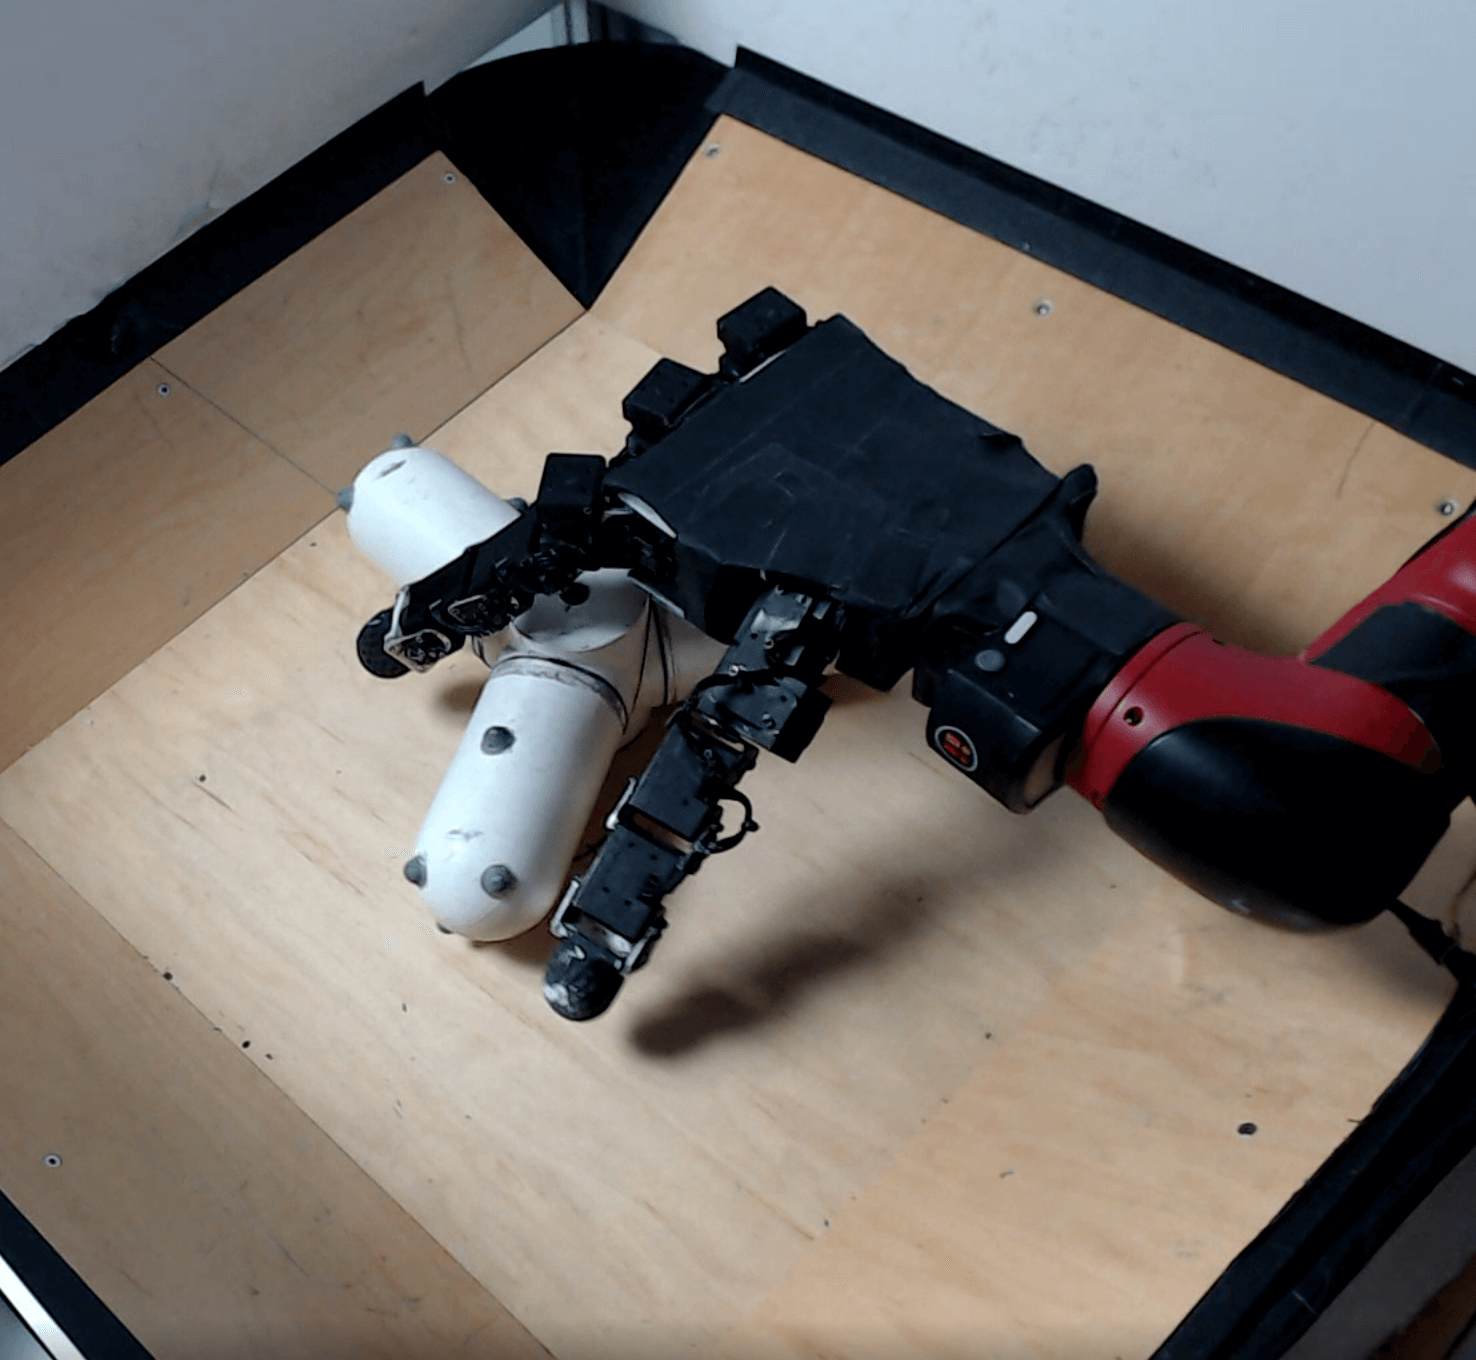
\includegraphics[height=0.6\textwidth]{awac/figures/robot/hand.png}
    %     % 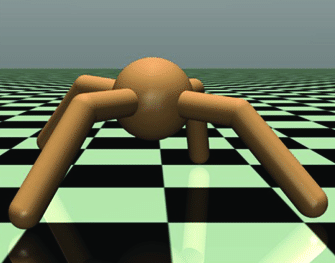
\includegraphics[height=0.26\textwidth]{awac/figures/imgs/ant.png}
    %     % 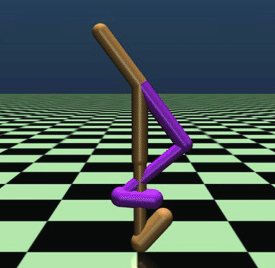
\includegraphics[height=0.26\textwidth]{awac/figures/imgs/walker.png}
    % \end{subfigure}
    % \begin{subfigure}[b]{0.3\textwidth}
    %     \center
    %     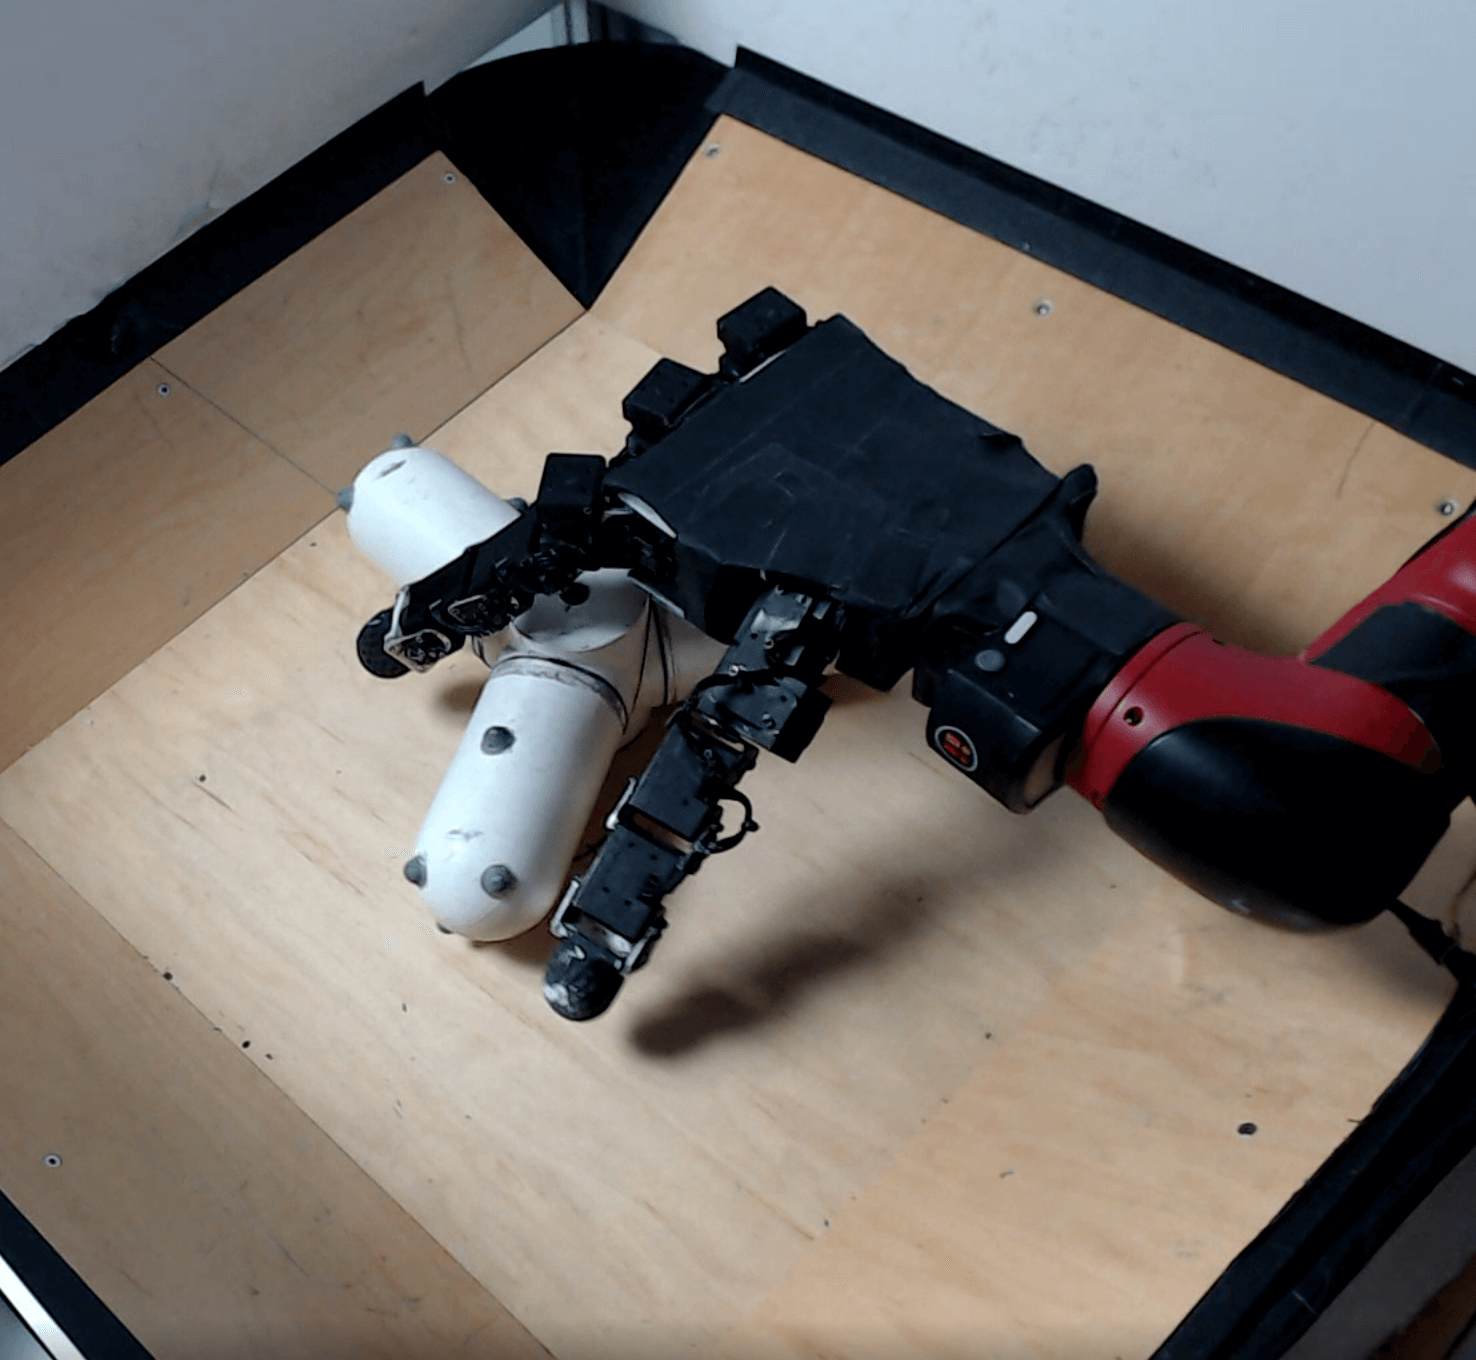
\includegraphics[height=0.6\textwidth]{awac/figures/robot/hand.png}
    % \end{subfigure}
    % \vspace{0.2cm}
    
    \centering
    \begin{subfigure}[b]{0.02\textwidth}
        \center
        \begin{turn}{90} 
            \footnotesize
            Average Return
        \end{turn}
        \vspace{0.8cm}
    \end{subfigure}
    \begin{subfigure}[b]{0.28\textwidth}
        \center
        % 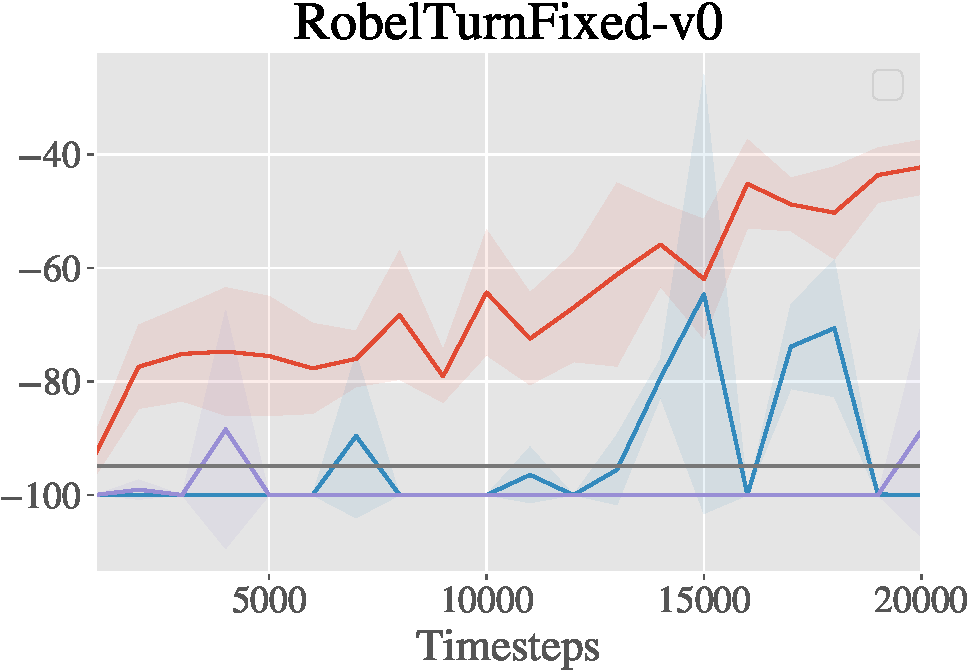
\includegraphics[height=1.15in]{awac/figures/robot/dclaw_curve-crop.pdf}
        % 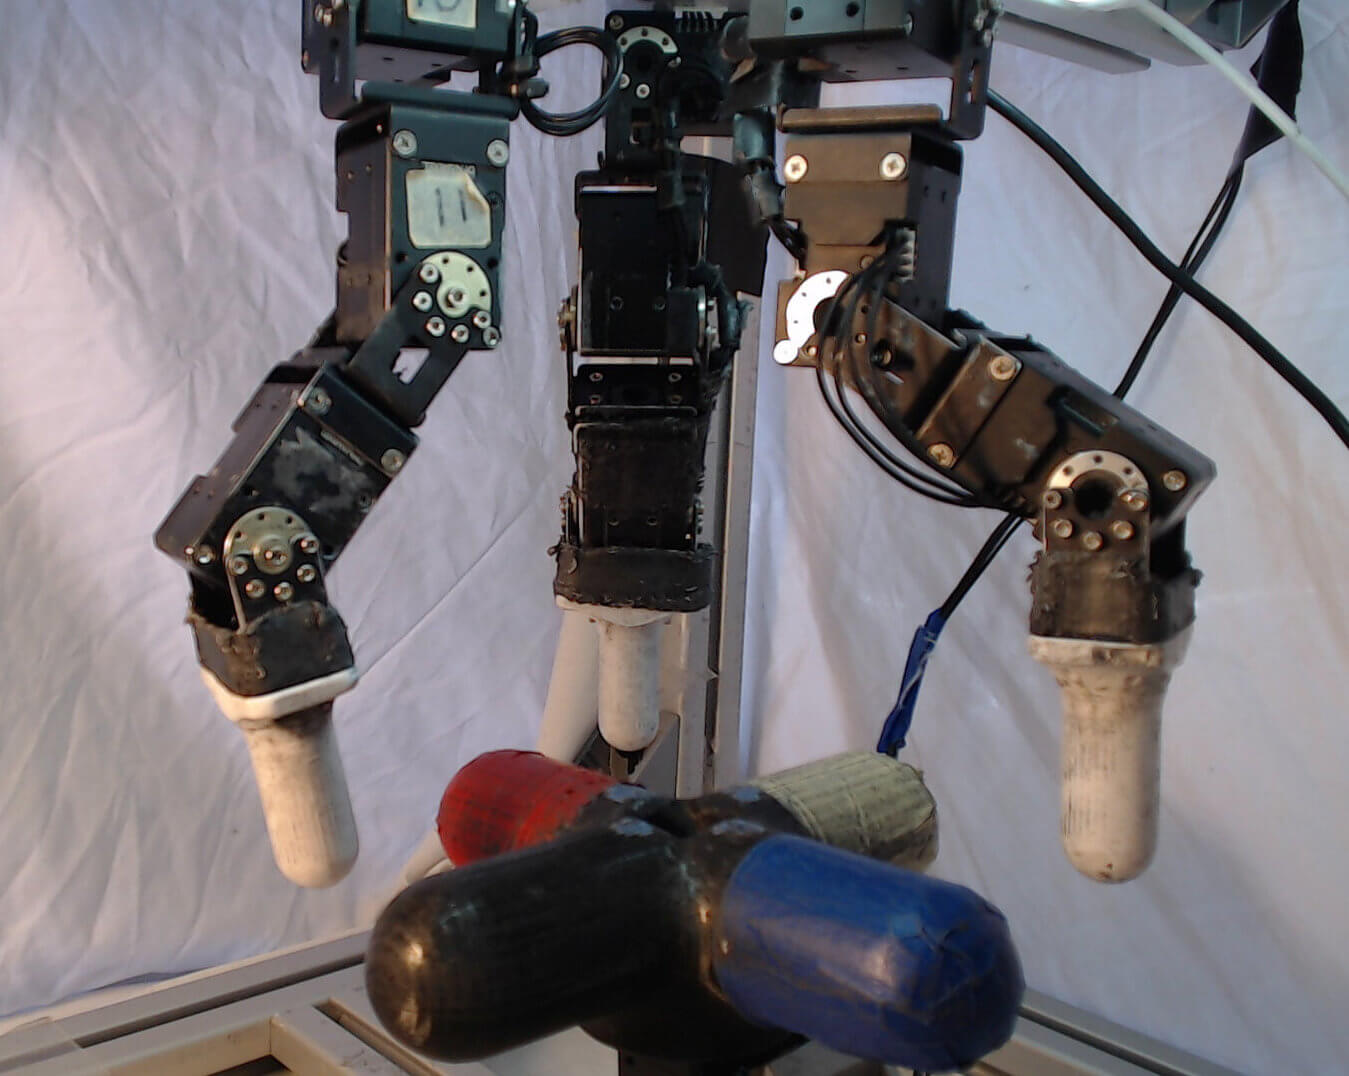
\includegraphics[height=0.4\textwidth]{awac/figures/robot/dclaw_new.jpg}
        % \vspace{0.3cm}
        
        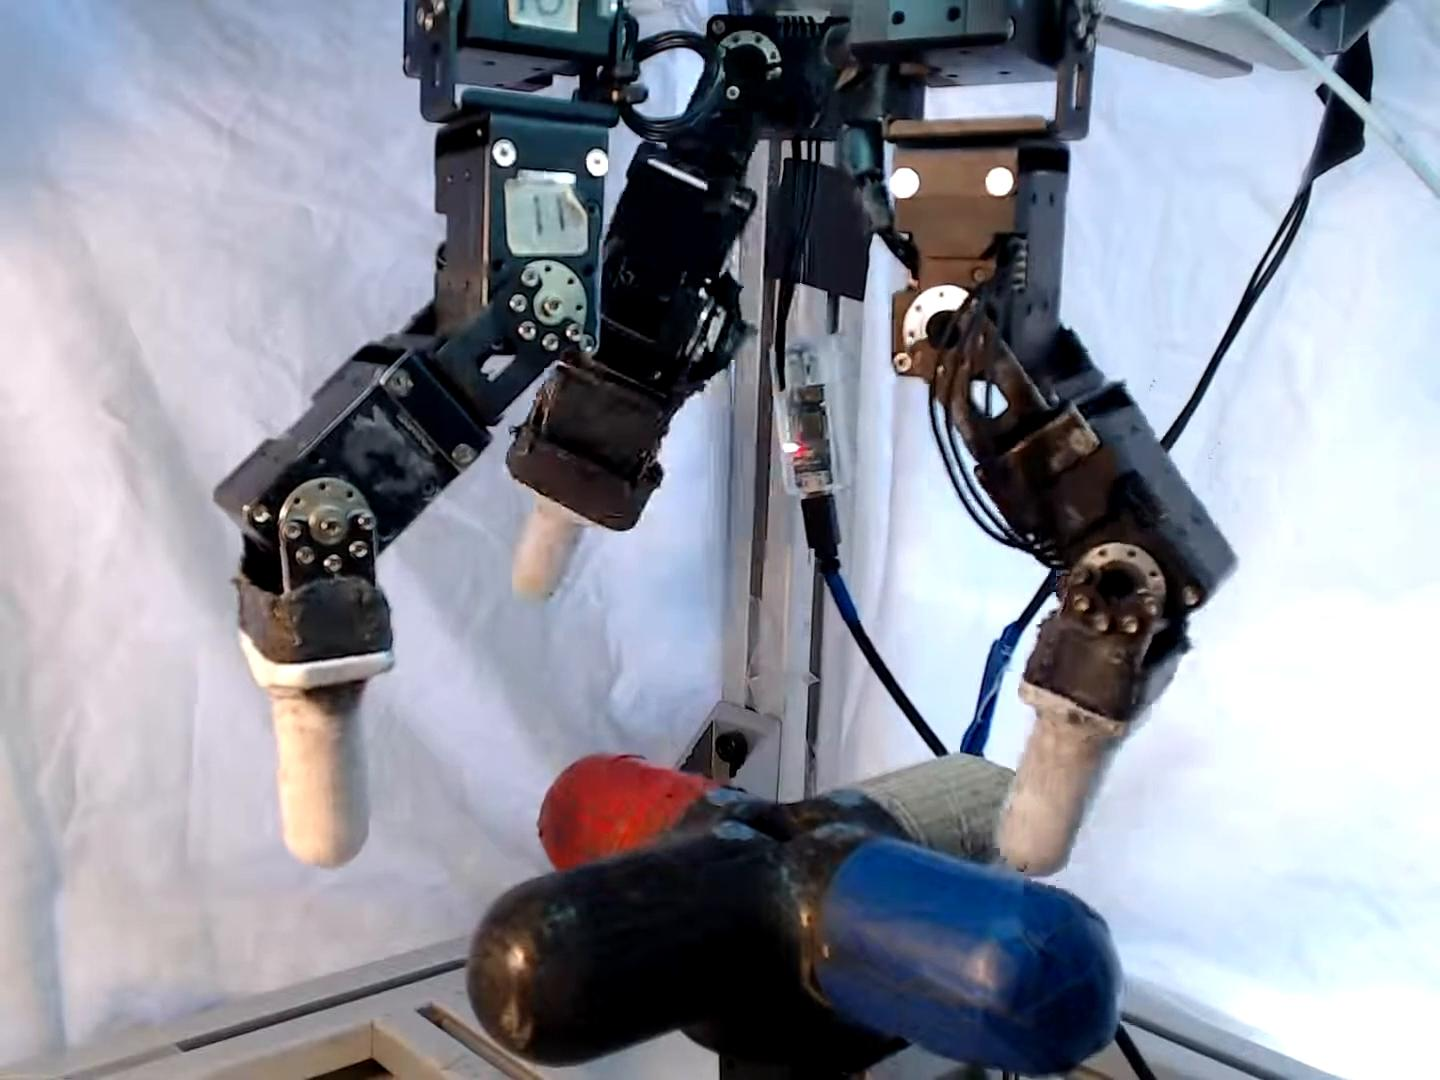
\includegraphics[height=0.22\linewidth]{awac/figures/filmstrip_claw/claw_vid_100.jpg}
        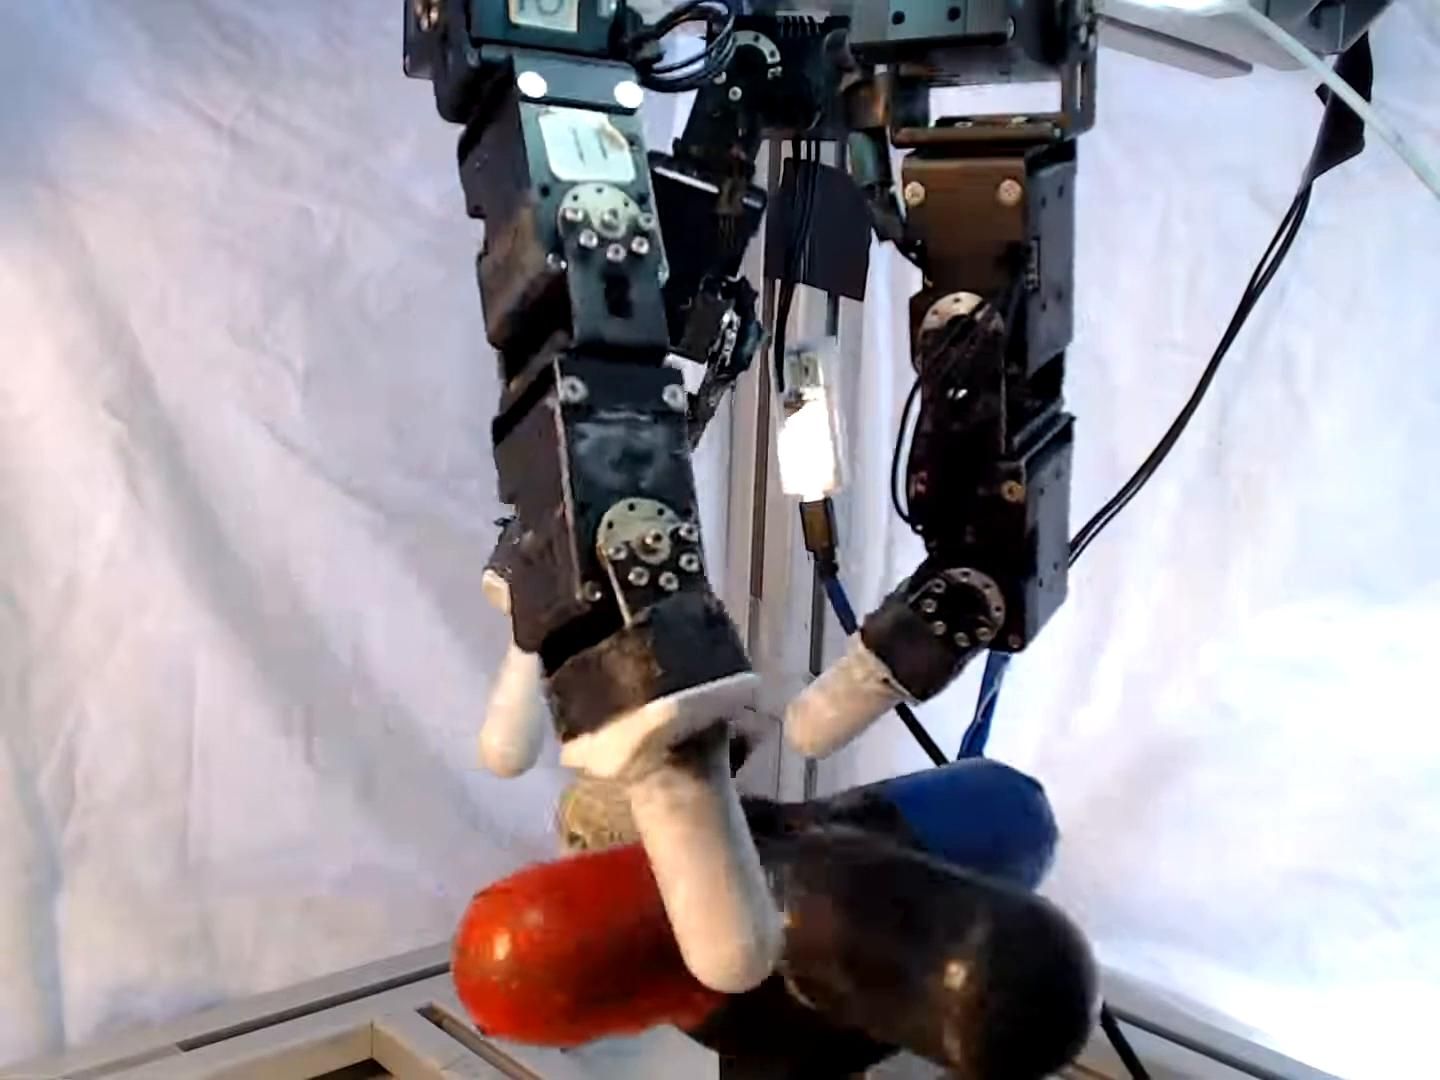
\includegraphics[height=0.22\linewidth]{awac/figures/filmstrip_claw/claw_vid_300.jpg}
        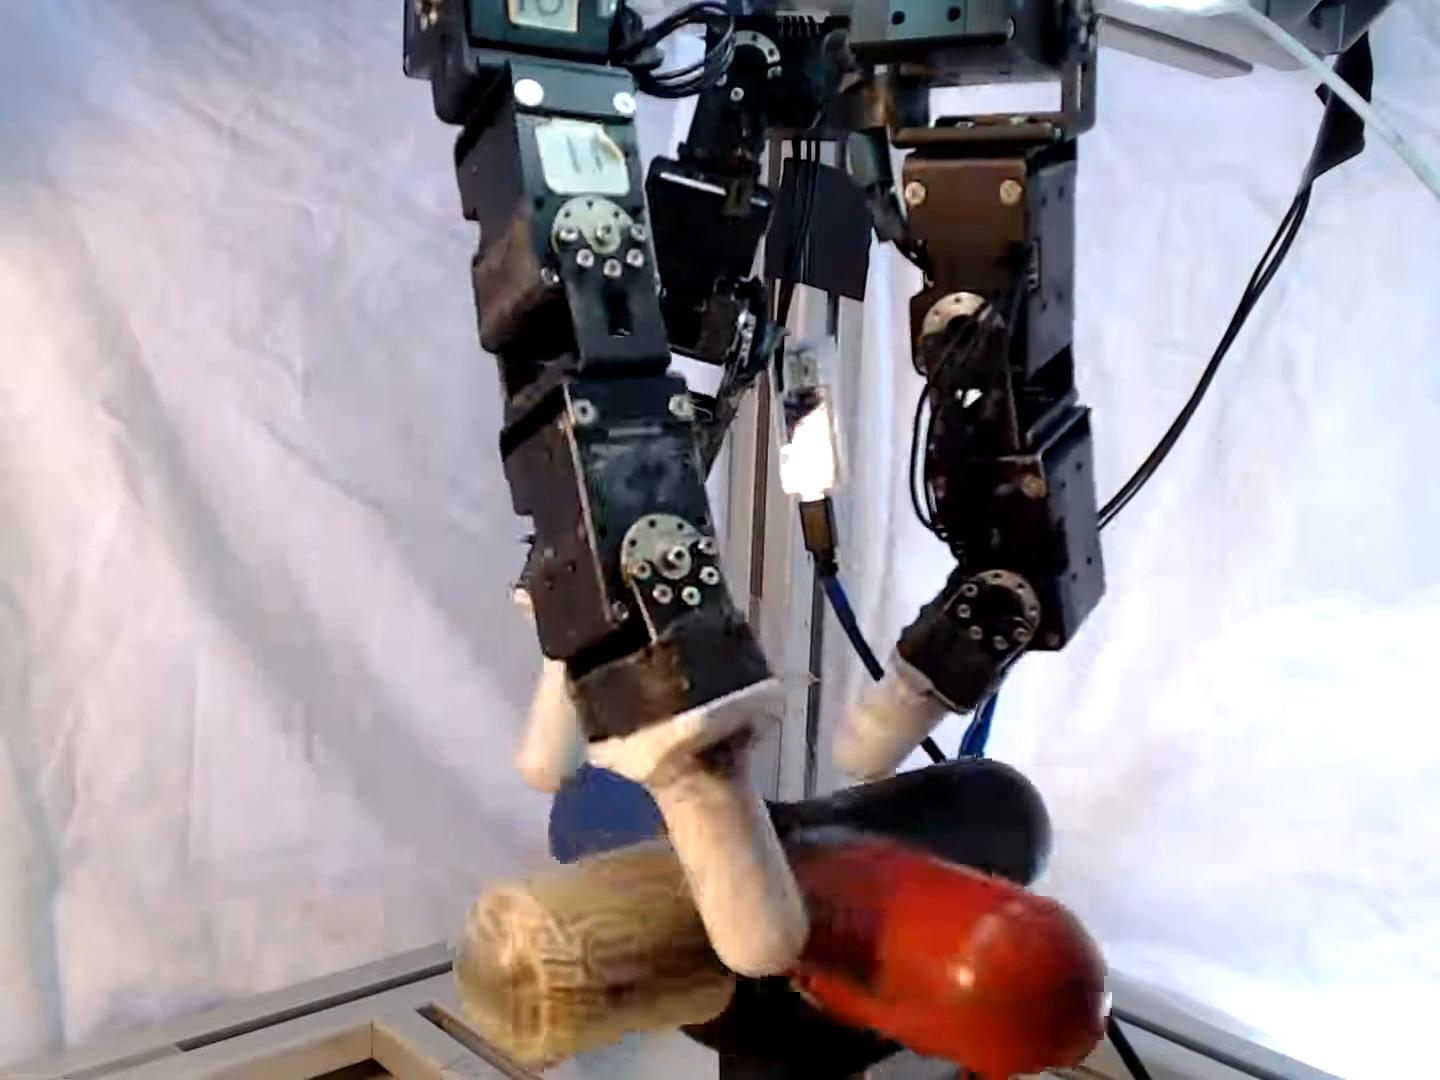
\includegraphics[height=0.22\linewidth]{awac/figures/filmstrip_claw/claw_vid_400.jpg}
        \vspace{0.1cm}

        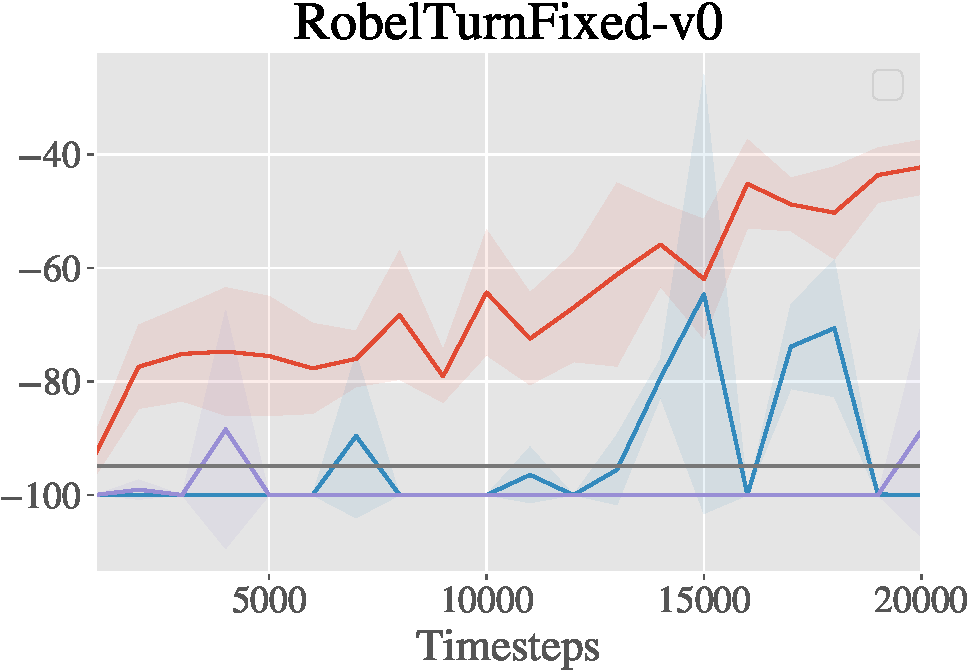
\includegraphics[width=0.99\textwidth]{awac/figures/robot/dclaw_curve-crop.pdf}
    \end{subfigure}
    \begin{subfigure}[b]{0.28\textwidth}
        \center
        % 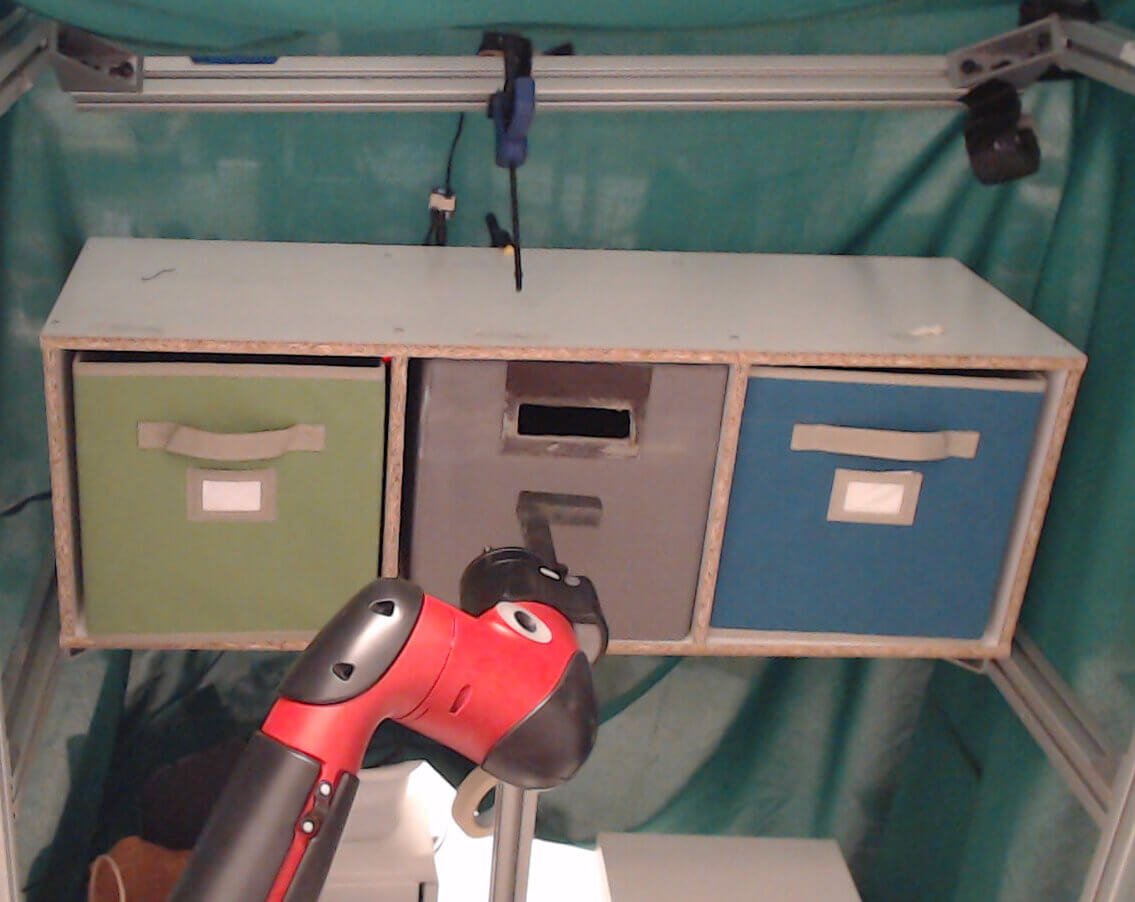
\includegraphics[height=0.4\textwidth]{awac/figures/robot/drawer_img.jpeg}
        % \vspace{0.3cm}
        
        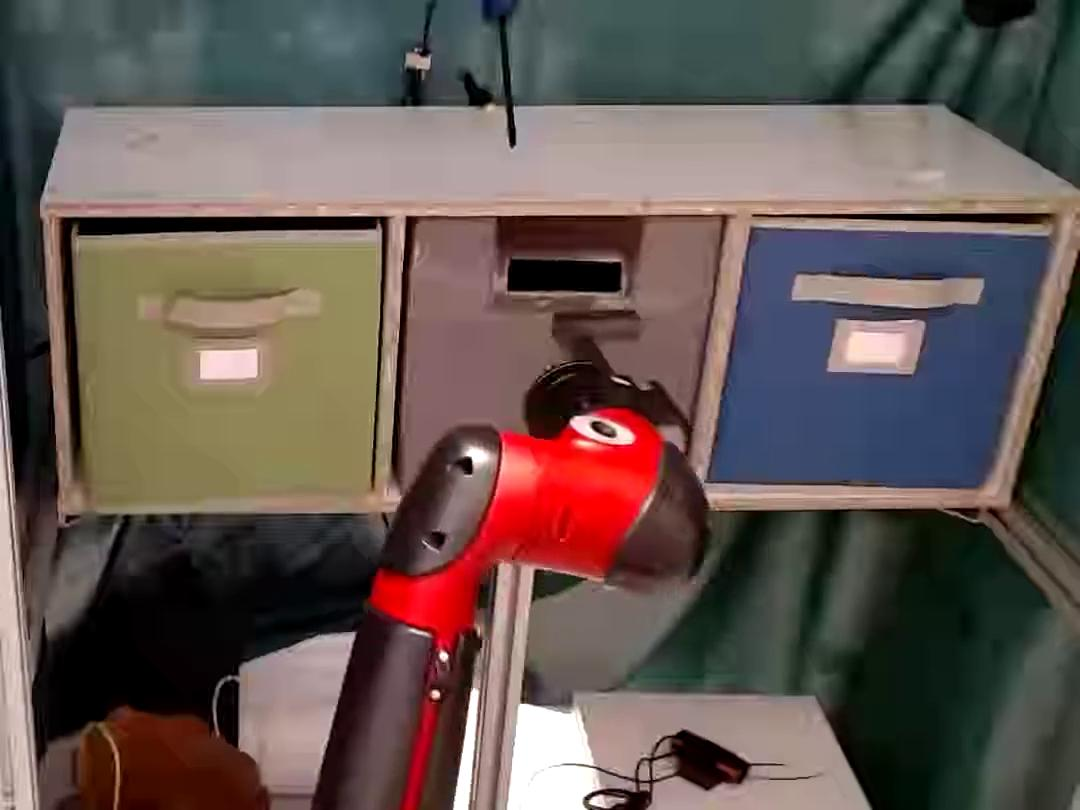
\includegraphics[height=0.22\linewidth]{awac/figures/filmstrip_drawer/drawer_vid_100.jpg}
        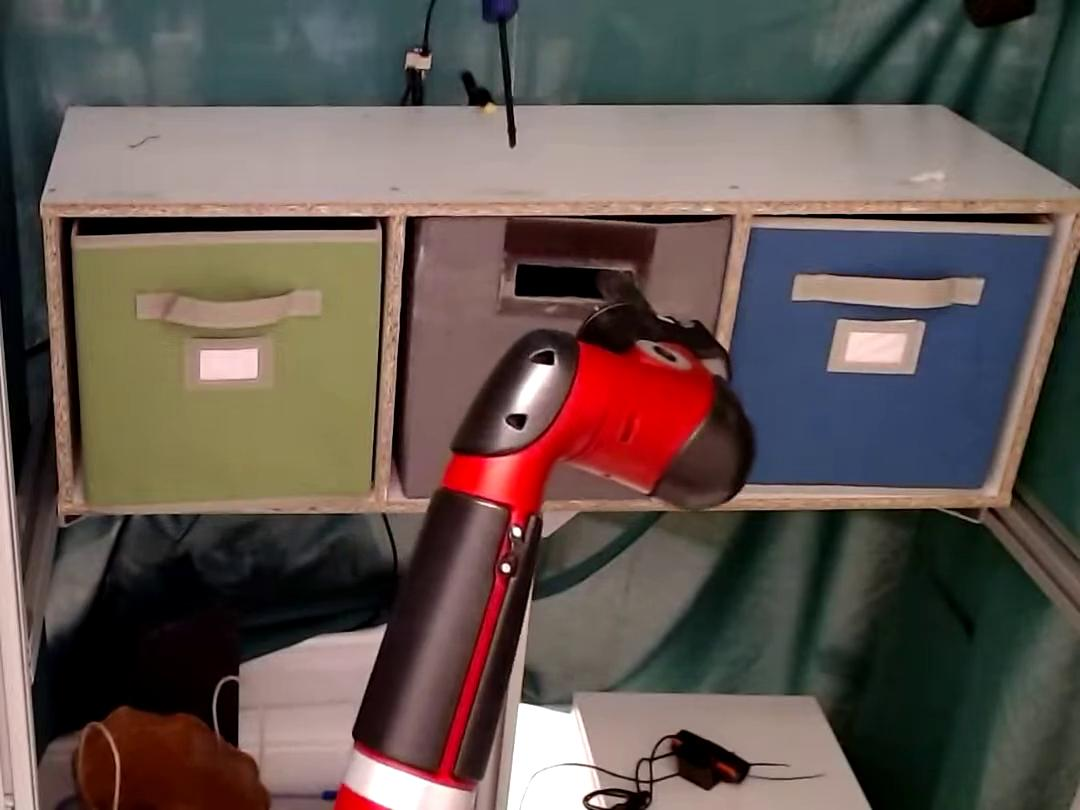
\includegraphics[height=0.22\linewidth]{awac/figures/filmstrip_drawer/drawer_vid_1100.jpg}
        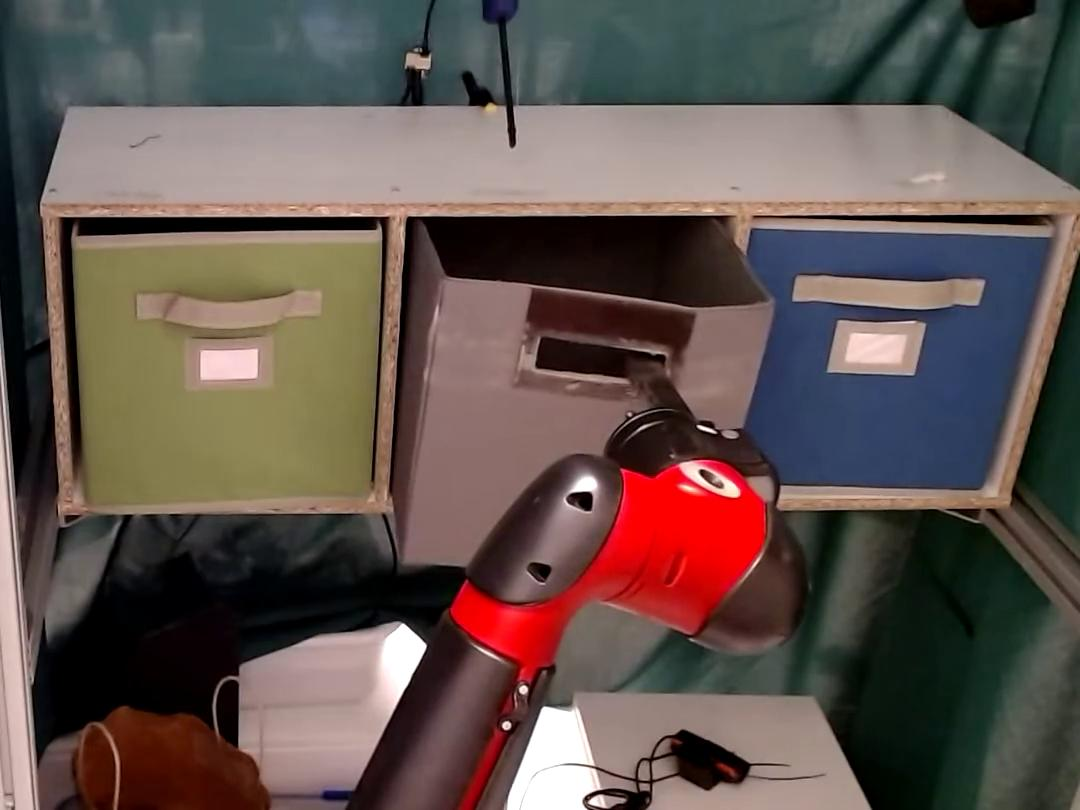
\includegraphics[height=0.22\linewidth]{awac/figures/filmstrip_drawer/drawer_vid_2900.jpg}
        \vspace{0.1cm}

        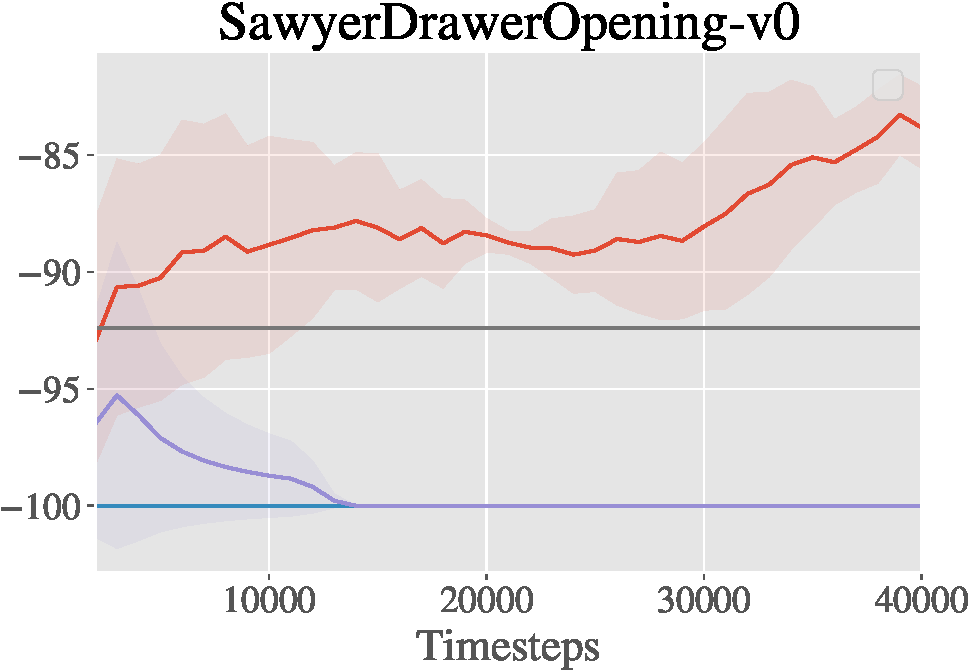
\includegraphics[width=0.99\textwidth]{awac/figures/robot/drawer_curve-crop.pdf}
    \end{subfigure}
    \begin{subfigure}[b]{0.28\textwidth}
        \center
        % 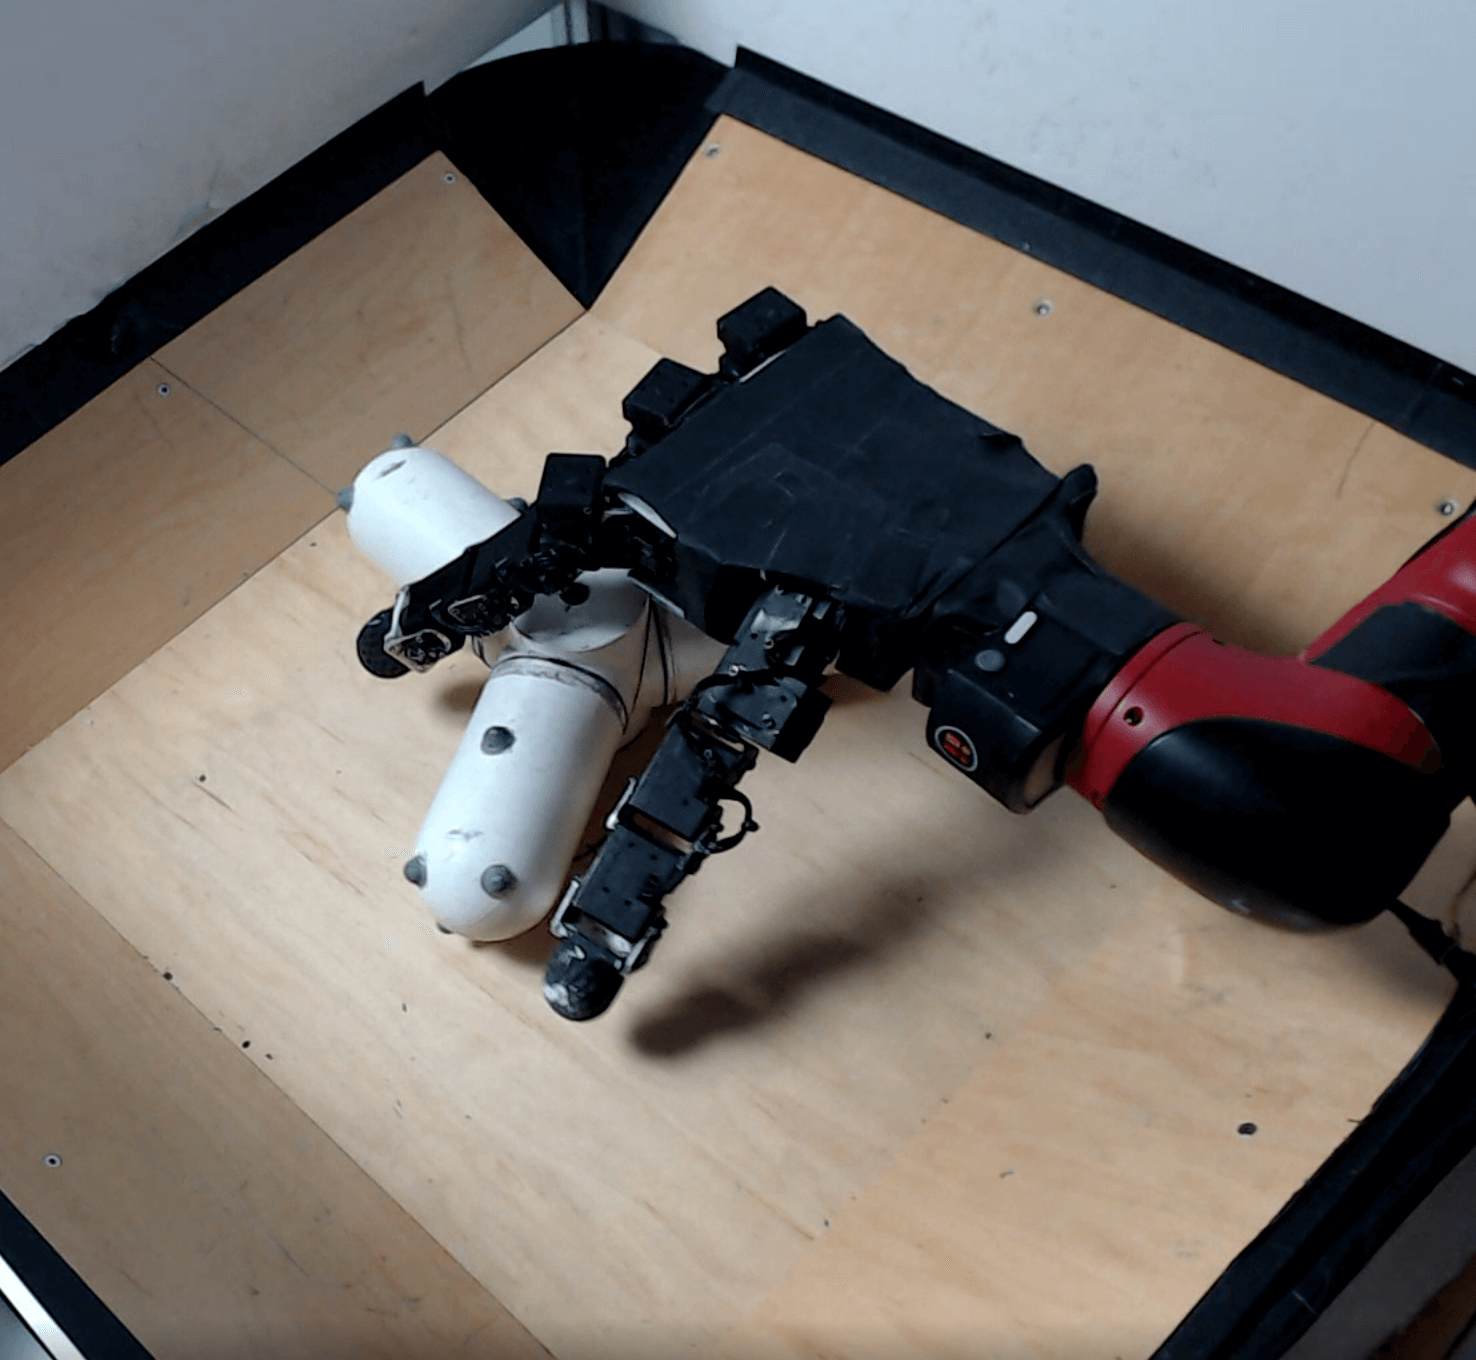
\includegraphics[height=0.4\textwidth]{awac/figures/robot/hand.png} \\
        % \vspace{0.3cm}
        \hspace{0.02\linewidth}
        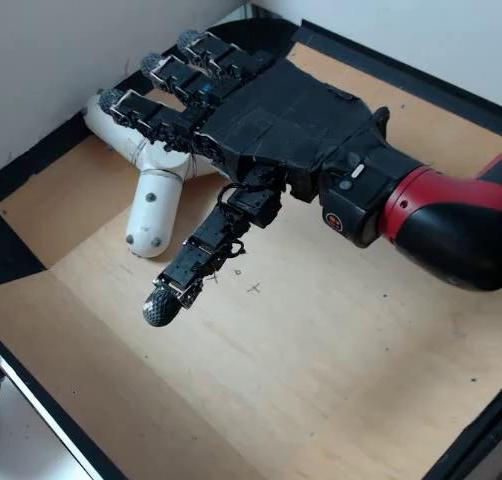
\includegraphics[height=0.22\linewidth]{awac/figures/filmstrip_hand/vid_0.jpg}
        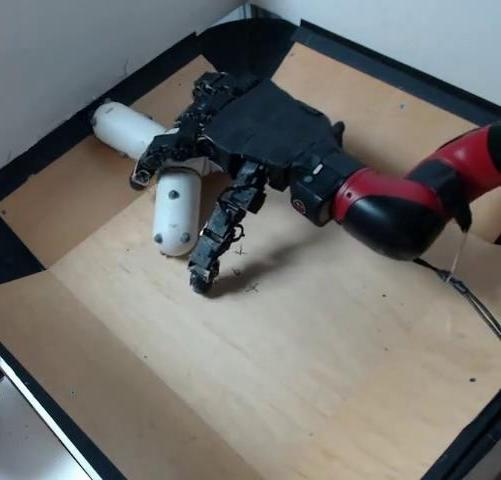
\includegraphics[height=0.22\linewidth]{awac/figures/filmstrip_hand/vid_70.jpg}
        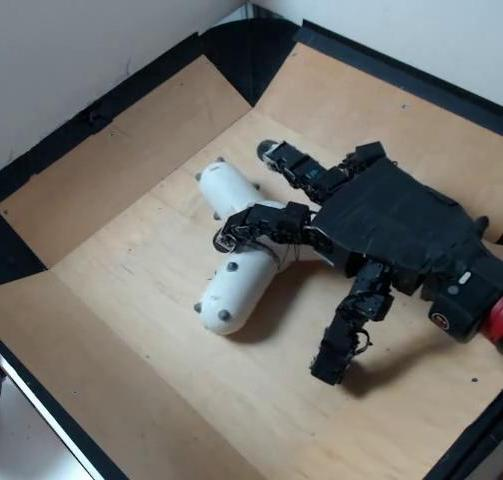
\includegraphics[height=0.22\linewidth]{awac/figures/filmstrip_hand/vid_190.jpg}
            \vspace{0.1cm}

        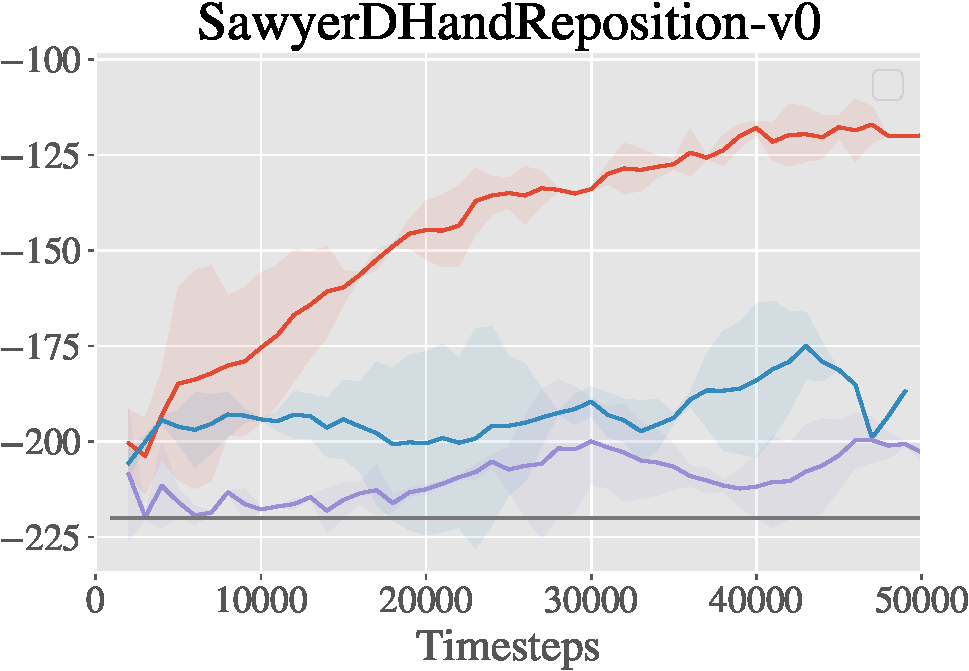
\includegraphics[width=0.99\textwidth]{awac/figures/robot/hand_curve-crop.pdf}
    \end{subfigure}
    \begin{subfigure}[b]{0.1\textwidth}
        \center
        \hspace{0.02\linewidth}
        % 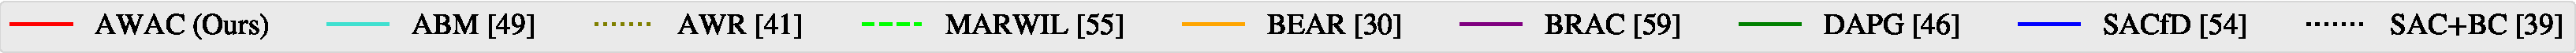
\includegraphics[width=1\textwidth]{awac/figures/mujoco/legend_ncol1-crop.pdf}
        % 
\includegraphics[width=0.5\textwidth]{awac/figures/robot/robot_legend-crop.pdf}
        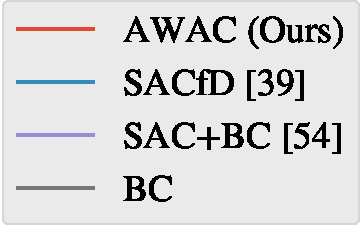
\includegraphics[width=0.99\textwidth]{awac/figures/robot/robot_legend4-crop.pdf}
        \vspace{0.6cm}
    \end{subfigure}

    \caption{
    % \footnotesize{
    Algorithm comparison on three real-world robotic environments. Images of real world robotic tasks are pictured above. Left: a three fingered D'claw must rotate a valve $180^\circ$. Middle: a Sawyer robot must slide open a drawer using a hook attachment. Right: a dexterous hand attached to a Sawyer robot must re-position an object to to the center of the table. On each task, AWAC trained offline achieves reasonable performance (shown at timestep 0) and then steadily improves from online interaction. Other methods, which also all have access to prior data, fail to utilize the prior data effectively offline and therefore exhibit slow or no online improvement. Videos of all experiments are available at \projectpage
    % ABM \cite{siegel2020abm} AWR \cite{peng2019awr} BEAR \cite{kumar19bear} BRAC \cite{wu2019brac} DAPG \cite{rajeswaran2018dextrous} SACfD \cite{vecerik17ddpgfd} SAC+BC \cite{nair2018demonstrations}
    % }
    %\vspace{-0.5cm}
    }
    \label{fig:robot-learning-curves}
\end{figure*}
